\documentclass[../../main.tex]{subfiles}
\graphicspath{{\subfix{../../image/}}} % 指定图片目录,后续可以直接使用图片文件名。

% 例如:
% \begin{figure}[H]
% \centering
% \includegraphics[scale=0.4]{图.png}
% \caption{}
% \label{figure:图}
% \end{figure}
% 注意:上述\label{}一定要放在\caption{}之后,否则引用图片序号会只会显示??.

\begin{document}

\section{二元运算与同余关系}

\begin{definition}
设 \( A \) 是一个集合. \( A \times A \) 到 \( A \) 的一个映射 \( \varphi \), 称为 \( A \) 的一个\textbf{二元运算}.

若记 \( \varphi(a,b) = ab \), 则称 \( ab \) 为 \( a \) 与 \( b \) 的\textbf{积}. 若记 \( \varphi(a,b) = a + b \), 则称 \( a + b \) 为 \( a \) 与 \( b \) 的\textbf{和}.

若 \( A \) 上的二元运算 \( \varphi(a,b) = ab \) 满足结合律
\[
(ab)c = a(bc),\quad \forall a,b,c \in A,
\]
则此二元运算称为\textbf{结合的}.

若 \( A \) 上的二元运算 \( \varphi(a,b) = ab \) 满足交换律
\[
ab = ba,\quad \forall a,b \in A,
\]
则此二元运算称为\textbf{交换的}. 一般地, 若 \( c,d \in A \) 有 \( cd = dc \), 则称 \( c \) 与 \( d \) 是\textbf{交换的}.
\end{definition}

\begin{definition}
设集合 \( A \) 有二元运算 \( (a,b) \to ab \) 且满足结合律, 则对 \( \forall n \in \mathbf{N} \) (\( \mathbf{N} \) 表示自然数, 即正整数的集合), 定义
\[
a^1 = a,\quad a^{n + 1} = a^n \cdot a,\quad \forall a \in A,
\]
\( a^n \) 称为 \( a \) 的  \( \boldsymbol{n} \) \textbf{次乘幂}, 也简称 \( \boldsymbol{n} \) \textbf{次幂}.

在 \( A \) 中也可以定义\textbf{连乘积}
\[
\prod_{i = 1}^n a_i = \left( \prod_{i = 1}^{n - 1} a_i \right) a_n,\quad a_i \in A, i = 1,2,\cdots, n.
\]
\end{definition}

\begin{proposition}\label{proposition:乘幂和连乘积的性质}
\begin{enumerate}
\item \( a^n a^m = a^{n + m}, (a^m)^n = a^{nm} (\forall a \in A, m,n \in \mathbf{N}) \). 

\item 若 \( a,b \in A \) 且 \( ab = ba \), 则 \( (ab)^n = a^n b^n (\forall n \in \mathbf{N}) \).

\item 若有
\[
0 = n_0 < n_1 < \cdots < n_r = n,
\]
则
\[
\prod_{j = 1}^r \left( \prod_{k = n_{j - 1} + 1}^{n_j} a_k \right) = \prod_{i = 1}^n a_i.
\]
\end{enumerate}
\end{proposition}
\begin{proof}
证明是显然的.
\end{proof}

\begin{definition}
如果将二元运算记为加法且满足结合律, 于是可定义\textbf{倍数}与\textbf{连加}如下:
\[
1 \cdot a = a,\quad (n + 1)a = na + a,
\]
\[
\sum_{i = 1}^n a_i = \left( \sum_{i = 1}^{n - 1} a_i \right) + a_n.
\]
\end{definition}

\begin{proposition}\label{proposition:倍数和连加的性质}
\begin{enumerate}
\item $na + ma = (n + m)a,\quad n(ma) = (nm)a,\quad \forall a \in A, m,n \in \mathbf{N}.$

\item 若 \( a + b = b + a \), 则
\[
n(a + b) = na + nb,\quad \forall n \in \mathbf{N},
\]

\item 若有
\[
0 = n_0 < n_1 < \cdots < n_r = n,
\]
则
\[
\sum_{j = 1}^r \left( \sum_{k = n_{j - 1} + 1}^{n_j} a_k \right) = \sum_{i = 1}^n a_i.
\]
\end{enumerate}
\end{proposition}
\begin{proof}
证明是显然的.
\end{proof}

\begin{definition}[(二元)关系]
所谓在集合 \( A \) 中定义了二元素间的一个\textbf{(二元)关系} \( R \), 也就是给出了集合 \( A \times A \) 中元素的一个性质 \( R \), 若 \( a,b \in A \), \( (a,b) \) 有性质 \( R \), 则称 \( a \) 与 \( b \) 有关系 \( R \), 记为 \( aRb \).
\end{definition}
\begin{note}
事实上, 集合 \( A \) 中关系 \( R \) 可由 \( A \times A \) 中子集
\[
S \triangleq  \{(a,b) \mid a,b \in A, aRb\}
\]
来刻画.即若$aRb$,则$(a,b)\in S.$

反之, 由 \( A \times A \) 的一个子集 \( S \), 也可确定 \( A \) 一个关系$R$.即若 \( (a,b) \in S \),则 \( aRb \).
\end{note}

\begin{definition}[等价关系]
\begin{enumerate}
\item 集合 \( A \) 中关系若满足以下条件:
\begin{enumerate}[(1)]
\item \textbf{自反性} \( aRa, \forall a \in A \);

\item \textbf{对称性} 若 \( aRb \), 则 \( bRa \);

\item \textbf{传递性} 若 \( aRb, bRc \), 则 \( aRc \),
\end{enumerate}
则称 \( R \) 为 \( A \) 的一个\textbf{等价关系}.

\item 若仍以 \( R \) 表示 \( A \) 中关系所确定的 \( A \times A \) 的子集, 则 \( R \) 为等价关系当且仅当下列三个条件同时成立:
\begin{enumerate}[(1)]
\item \( (a,a) \in R, \forall a \in A \);

\item 若 \( (a,b) \in R \), 则 \( (b,a) \in R \);

\item 若 \( (a,b) \in R, (b,c) \in R \), 则 \( (a,c) \in R \).
\end{enumerate}
\end{enumerate}
\end{definition}
\begin{remark}
在等价关系定义中的三个条件是互相独立的,缺一不可.
\end{remark}

\begin{definition}[等价类和代表元素]
若 \( R \) 是集合 \( A \) 的一个等价关系且 \( a \in A \), 则 \( A \) 中所有与 \( a \) 有关系 \( R \) 的元素集合
\[
K_a = \{ b \in A \mid bRa \}
\]
称为 \( a \) 所在的\textbf{等价类}, \( a \) 称为这个等价类的\textbf{代表元素}.
\end{definition}

\begin{definition}[分划/分类]
集合 \( A \) 的一个子集族 \( \{ A_\alpha \} \) 称为 \( A \) 的一个\textbf{分划}或\textbf{分类}, 如果满足
\[
A = \bigcup_\alpha A_\alpha,\quad A_\alpha \bigcap A_\beta = \varnothing,\quad \text{若 } \alpha \neq \beta.
\]
也称 \( A \) 是 \( \{ A_\alpha \} \) 中\textbf{所有不相交的集合的并}或\textbf{无交并}.
\end{definition}

\begin{theorem}\label{theorem:等价类就和集合的分划对应}
设 \( R \) 是集合 \( A \) 的等价关系, 则由所有不同的等价类构成的子集族 \( \{ K_a \} \) 是 \( A \) 的分划. 

反之, 若 \( \{ A_a \} \) 是 \( A \) 的分划, 则可在 \( A \) 中定义等价关系$R$,
\[
aRb, \quad \text{若 } \exists A_\alpha, \text{使 } a,b \in A_\alpha.
\]
并且使得每个 \( A_a \) 是一等价类.
\end{theorem}
\begin{proof}
设 \( R \) 是 \( A \) 的等价关系. 由 \( \forall a \in A, aRa \) 知 \( a \in K_a \), 于是 \( A = \bigcup_a K_a \). 设 \( K_a \cap K_b \neq \varnothing \), 即 \( \exists c \in K_a \cap K_b \), 对 \( \forall x \in K_a \) 有 \( cRa, xRa \), 因而 \( xRc \). 又 \( cRb \), 故 \( xRb \), 即 \( x \in K_b \), 从而得 \( K_a \subseteq K_b \). 同样可得 \( K_b \subseteq K_a \), 故 \( K_a = K_b \), 亦即若 \( K_a \neq K_b \), 则 \( K_a \cap K_b = \varnothing \). 这样就证明了 \( \{ K_a \} \) 是 \( A \) 的分划.

反之, 设 \( \{ A_\alpha \} \) 是 \( A \) 的一个分划. 在 \( A \) 中定义关系 \( R \),
\[
aRb, \quad \text{若 } \exists A_\alpha, \text{使 } a,b \in A_\alpha.
\]
因 \( A = \bigcup_\alpha A_\alpha \), 故对 \( \forall a \in A, \exists A_\alpha \), 使 \( a \in A_\alpha \), 因此 \( a,a \in A_\alpha \), 即 \( aRa \). 其次, 若 \( aRb \), 即 \( \exists A_\alpha \), 使 \( a,b \in A_\alpha \). 自然 \( b,a \in A_\alpha \), 故 \( bRa \). 再次, 若 \( aRb, bRc \), 即有 \( A_\alpha, A_\beta \), 使 \( a,b \in A_\alpha \) 且 \( b,c \in A_\beta \), 故 \( b \in A_\alpha \cap A_\beta \). 由 \( \{ A_\alpha \} \) 为 \( A \) 的分划知 \( A_\alpha = A_\beta \), 因而 \( aRc \). 这样就证明了 \( R \) 是等价关系. 由 \( R \) 的定义知若 \( a \in A_\alpha \), 则$a$所在的等价类\( K_a = A_\alpha \).
\end{proof}

\begin{definition}[商集和自然映射]
设 \( R \) 是集合 \( A \) 的等价关系. 以关于 \( R \) 的等价类为元素的集合 \( \{ K_a \} \) 称为 \( A \) 对 \( R \) 的\textbf{商集合}或\textbf{商集}. 记为 \( A/R \). 由
\[
\pi(a) = K_a,\quad \forall a \in A 
\]
定义的 \( A \) 到 \( A/R \) 上的映射 \( \pi \) 称为 \( A \) 到 \( A/R \) 上的\textbf{自然映射}.
\end{definition}

\begin{theorem}\label{theorem:一个满射可定义一个等价关系}
设 \( f:A \to B \) 是满映射. 在 \( A \) 中定义关系 \( R \),
\[
aRb,\quad \text{若 } f(a) = f(b),
\]
则 \( R \) 是 \( A \) 的等价关系. 又设 \( \pi:A \to A/R \) 为自然映射, 则有 \( A/R \) 到 \( B \) 上的一一对应 \( g \) 满足
\begin{align}
g\pi = f. \label{eq:::----4234211.1.8}
\end{align}
即\reffig{交换图1}是交换图.
\end{theorem}
\begin{figure}[H]
\centering
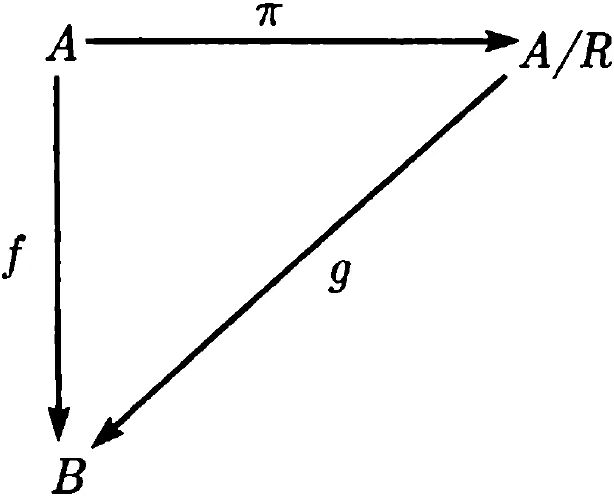
\includegraphics[scale=0.25]{交换图1.png}
\caption{}
\label{figure:交换图1}
\end{figure}
\begin{proof}
考虑 \( y \in B \) 的原像 \( f^{-1}(y) \) 构成的子集族. 显然, \( A = \bigcup_{y \in B} f^{-1}(y) \). 又若 \( y,z \in B \), \( f^{-1}(y) \cap f^{-1}(z) \neq \varnothing \), 即 \( \exists a \in A \), 使 \( f(a) = y, f(a) = z \), 即 \( y = z \). 故 \( f^{-1}(y) = f^{-1}(z) \), 从而 \( \{ f^{-1}(y) \} \) 是 \( A \) 的一个分划. 于是由\refthe{theorem:等价类就和集合的分划对应}知,在 \( A \) 中可定义等价关系 \( R: aRb \), 若 \( \exists f^{-1}(y) \), 使 \( a,b \in f^{-1}(y) \), 即 \( f(a) = f(b) \). 由此知定理的第一部分成立.

定义\( A/R \) 到 \( B \) 的映射 \( g \),
\[
g(K_a) = f(a),\quad \forall a \in A.
\]
注意到\( A \) 中元素 \( a \) 所在等价类 \( K_a = f^{-1}(f(a)) \), 由于 \( K_a = K_b \) 当且仅当 \( f(a) = f(b) \), 故$g$是单射.又 \( f(A) = B \), 故 \( g \) 是满射.因此$g$是一一对应. 由 \( \pi \) 的定义知式 \eqref{eq:::----4234211.1.8} 成立.
\end{proof}

\begin{definition}[同余关系和同余类]
设集合中 \( A \) 的二元运算, 记作乘法. 若 \( A \) 的一个等价关系 \( \sim \) 满足
\[
\text{若 } a \sim b, c \sim d, \text{ 则 } ac \sim bd, \forall a,b,c,d \in A .
\]
则称 \( \sim \) 为 \( A \) 的一个\textbf{同余关系}. \( a \in A \) 的等价类 \( K_a \) 此时也称为 \( a \) 的\textbf{同余类}.
\end{definition}

\begin{example}
\begin{enumerate}
\item 设 \( m \in \mathbf{Z} \)( 所有整数的集合 ), \( m \neq 0 \). 在 \( \mathbf{Z} \) 中定义关系
\[
a \sim b, \quad \text{若 } a \equiv b \pmod{m}.
\]
易证 \( \sim \) 是等价关系且由 \( a \equiv b \pmod{m} \), \( c \equiv d \pmod{m} \) 可得 \( a + c \equiv b + d \pmod{m} \), \( ac \equiv bd \pmod{m} \). 因而 \( \sim \) 对于 \( \mathbf{Z} \) 中的加法与乘法都是同余关系.

\item 设 \( \mathbf{P}[x] \) 是数域 \( \mathbf{P} \) 上一元多项式的集合. 设 \( f(x) \in \mathbf{P}[x] \), \( f(x) \neq 0 \). 在 \( \mathbf{P}[x] \) 中定义关系 \( \sim \): \( g(x) \sim h(x) \), 若 \( f(x) \mid (g(x) - h(x)) \). 与第一问类似可证 \( \sim \) 对 \( \mathbf{P}[x] \) 中的加法与乘法都是同余关系.

\item 以 \( \mathbf{P}^{n \times n} \) 表示数域 \( \mathbf{P} \) 上所有 \( n \) 阶方阵的集合. 方阵的加法与乘法都是 \( \mathbf{P}^{n \times n} \) 中的二元运算. 对 \( \boldsymbol{A} \in \mathbf{P}^{n \times n} \), 用 \( \text{ent}_{ij}\boldsymbol{A} \), \( \text{row}_i\boldsymbol{A} \), \( \text{col}_j\boldsymbol{A} \) 和 \( \det\boldsymbol{A} \) 分别表示 \( \boldsymbol{A} \) 的第 \( i \) 行第 \( j \) 列元素、\( \boldsymbol{A} \) 的第 \( i \) 行、\( \boldsymbol{A} \) 的第 \( j \) 列和 \( \boldsymbol{A} \) 的行列式.

\( \mathbf{P}^{n \times n} \) 中由 \( \det\boldsymbol{A} = \det\boldsymbol{B} \) 确定的关系, 对乘法是同余关系, 但对加法除 \( n = 1 \) 的情形外不是同余关系.
\end{enumerate}
\end{example}

\begin{theorem}\label{theorem:同余关系诱导商集中的乘法-定理1.1.3}
设集合 \( A \) 有二元运算乘法, \( \sim \) 是 \( A \) 的一个同余关系. 又 \( \pi: A \to A/\sim \) 是自然映射, 则在商集合 \( A/\sim \) 中可定义二元运算
\[
\pi(a)\pi(b) = \pi(ab),\quad \forall a,b \in A .
\]
\end{theorem}
\begin{proof}
要证明这个二元运算的良定义性,只需证由 \( \pi(a) = \pi(a_1) \), \( \pi(b) = \pi(b_1) \) 可得 \( \pi(ab) = \pi(a_1b_1) \), 其中, \( a,b,a_1, b_1 \in A \). 事实上, 由 \( \pi \) 的定义知 \( \pi(a) = \pi(a_1) \), 即 \( a \sim a_1 \), \( \pi(b) = \pi(b_1) \), 即 \( b \sim b_1 \). 因 \( \sim \) 是同余关系, 故 \( ab \sim a_1b_1 \), 所以 \( \pi(ab) = \pi(a_1b_1) \).
\end{proof}






























\end{document}